%----------------------------------------------------------------------------------------
%    PACKAGES AND THEMES
%----------------------------------------------------------------------------------------

\documentclass[aspectratio=169,xcolor=dvipsnames]{beamer}
\usetheme{SimpleDarkBlue}

\usepackage{hyperref}
\usepackage{graphicx}
\usepackage{booktabs}

\usepackage{fontspec}
\usepackage{luatexja}
\usepackage{appendixnumberbeamer}

% --- Math / figures (added, compatible with your template) ---
\usepackage{amsmath, amssymb, bm}
\usepackage{tikz}
\usetikzlibrary{positioning, arrows.meta, shapes.misc}

\setmainfont{Alegreya Sans Light}[
  ItalicFont={* Italic},
  BoldFont={Alegreya Sans Medium},
  BoldItalicFont={Alegreya Sans Medium Italic}]
\setsansfont{Alegreya Sans Light}[
  ItalicFont={* Italic},
  BoldFont={Alegreya Sans Medium},
  BoldItalicFont={Alegreya Sans Medium Italic}]

% ------------ %
% beamerbutton %
% ------------ %
\newcommand{\goto}[2]{\hyperlink{#2}{\beamergotobutton{#1}}}
\newcommand{\return}[2]{\hyperlink{#2}{\beamerreturnbutton{#1}}}
\newcommand{\extgoto}[2]{\href{#2}{\beamergotobutton{#1}}}

% ------------------------------------ %
% Section title page with Huge bf text %
% ------------------------------------ %
\AtBeginSection[]{
  \begin{frame}[noframenumbering, plain]
    \Huge{\centerline{\textbf{\insertsection}}}
  \end{frame}
}

%%% automatically add spaces into enumerate and itemize environment
\let\tempone\itemize
\let\temptwo\enditemize
\renewenvironment{itemize}{\tempone\addtolength{\itemsep}{\fill}}{\temptwo}
\let\tempa\enumerate
\let\tempb\endenumerate
\renewenvironment{enumerate}{\tempa\addtolength{\itemsep}{\fill}}{\tempb}

%%=============================================================
%%  FOOTLINE TEMPLATE
%%=============================================================
\defbeamertemplate*{footline}{shadow theme}{%
    \leavevmode\hbox{%
        \hypersetup{linkcolor=white,urlcolor=white,citecolor=white}
        \begin{beamercolorbox}[wd=1.02\paperwidth, ht=2.5ex, dp=1.125ex, leftskip=.3cm plus1fil, rightskip=0.3cm]{author in head/foot}%
            \insertsectionnavigationhorizontal{.80\textwidth}{}{} \hspace{.3cm} \hfill \#\ \insertframenumber \ / \ \inserttotalframenumber%
        \end{beamercolorbox}%
    }%
}
\setbeamertemplate{footline}[shadow theme]
\setbeamertemplate{navigation symbols}{}

% ----------------
% Helpful macros
% ----------------
\newcommand{\E}{\mathbb{E}}
\newcommand{\R}{\mathbb{R}}

%----------------------------------------------------------------------------------------
%    TITLE PAGE
%----------------------------------------------------------------------------------------

\title[Graduate Macro]{Graduate Macro Sequence:\\Roadmap and Motivation}
\author[Hui-Jun Chen]{Hui-Jun Chen}
\institute[]{
    National Tsing Hua University\\
    Department of Economics
    }\vspace{2pt}
\date{\today}

%----------------------------------------------------------------------------------------
%    PRESENTATION SLIDES
%----------------------------------------------------------------------------------------

\begin{document}

%------------------------------------------------
\begin{frame}[plain,noframenumbering]
    \titlepage
\end{frame}

%========================================================================================
\section[Why]{Why this sequence?}
%========================================================================================

\begin{frame}{What you will be able to do after this sequence}

\begin{itemize}
  \item Translate a macro question into \textbf{states}, \textbf{choices}, and \textbf{equilibrium conditions}
  \item Solve for \textbf{policy functions}, \textbf{prices}, and sometimes a \textbf{distribution}
  \item Use the model to run \textbf{counterfactuals} (policy, shocks, institutions)
  \item Read modern papers and quickly identify:
  \begin{itemize}
    \item what is new,
    \item what drives results,
    \item what is testable in data
  \end{itemize}
\end{itemize}
\end{frame}

\begin{frame}{The throughline: one language, many applications}

Across the entire course, we will repeatedly do:
\begin{enumerate}
  \item A \textbf{dynamic decision problem} \(\rightarrow\) policy rules
  \item \textbf{Equilibrium} \(\rightarrow\) market clearing, pricing, aggregation
  \item \textbf{Quantitative discipline} \(\rightarrow\) moments, impulse responses, counterfactuals
\end{enumerate}

\vspace{0.6em}
\small
Think of this as learning the \textbf{objects} of macro: policies, prices, and (sometimes) distributions.
\end{frame}

\begin{frame}{Course map (how the pieces fit)}
\centering
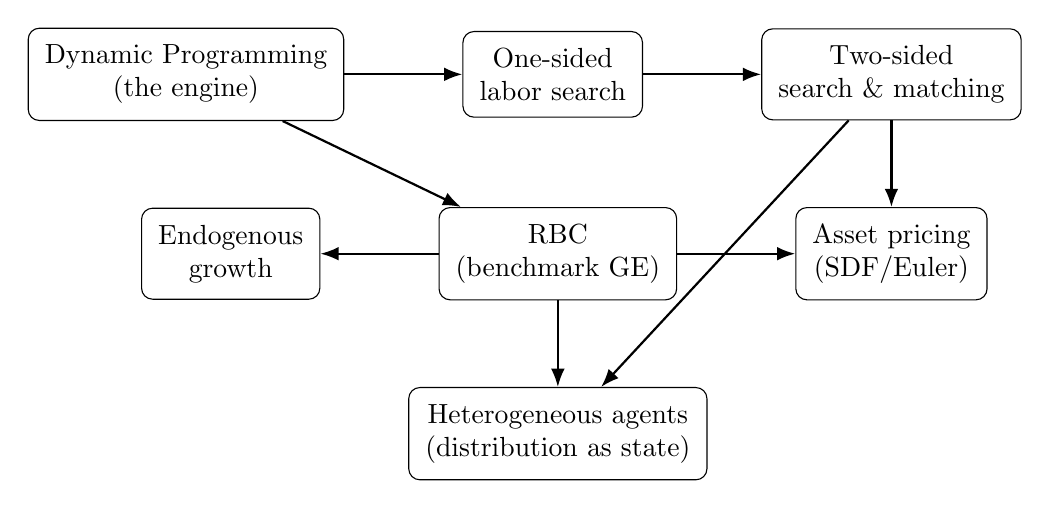
\begin{tikzpicture}[
  node/.style={rounded corners, draw, align=center, inner sep=6pt},
  arr/.style={-Latex, thick}
]
\node[node] (dp) {Dynamic Programming\\(the engine)};
\node[node, right=1.5cm of dp] (os) {One-sided\\labor search};
\node[node, right=1.5cm of os] (ts) {Two-sided\\search \& matching};
\node[node, below=1.1cm of ts] (ap) {Asset pricing\\(SDF/Euler)};
\node[node, left=1.5cm of ap] (rbc) {RBC\\(benchmark GE)};
\node[node, left=1.5cm of rbc] (gr) {Endogenous\\growth};
\node[node, below=1.1cm of rbc] (ha) {Heterogeneous agents\\(distribution as state)};

\draw[arr] (dp) -- (os);
\draw[arr] (os) -- (ts);
\draw[arr] (ts) -- (ap);
\draw[arr] (dp) -- (rbc);
\draw[arr] (rbc) -- (ap);
\draw[arr] (rbc) -- (gr);
\draw[arr] (rbc) -- (ha);
\draw[arr] (ts) -- (ha);
\end{tikzpicture}

\vspace{0.8em}
\small
We start simple, then add realism by adding \textbf{search frictions}, \textbf{risk pricing}, \textbf{growth forces}, and \textbf{heterogeneity}.
\end{frame}

\begin{frame}{Why start from models?}

Models are useful when they:
\begin{itemize}
  \item Turn a complicated environment into a \textbf{transparent mechanism}
  \item Produce \textbf{quantitative} implications (not just signs)
  \item Give a disciplined language for:
  \begin{itemize}
    \item decomposition (what drives fluctuations?),
    \item welfare (who gains/loses?),
    \item policy design (which margin matters?)
  \end{itemize}
\end{itemize}
\end{frame}

%========================================================================================
\section[DP]{Dynamic programming}
%========================================================================================

\begin{frame}{Dynamic programming: the recursive mindset}

A dynamic economic problem has four ingredients:
\[
\text{state }x_t,\quad
\text{choice }a_t,\quad
x_{t+1}=f(x_t,a_t,\varepsilon_{t+1}),\quad
\text{payoff }u(x_t,a_t).
\]

\vspace{0.6em}
\begin{itemize}
  \item \textbf{State} summarizes everything today that matters for tomorrow
  \item \textbf{Policy function} \(a_t=g(x_t)\) is what we want
  \item Recursion turns “infinite horizon” into a \textbf{stationary} problem
\end{itemize}
\end{frame}

\begin{frame}{The Bellman equation (what we solve)}

\[
V(x)=\max_{a\in\Gamma(x)}
\left\{
u(x,a)+\beta\,\E\!\left[V(x')\,\middle|\,x,a\right]
\right\},
\qquad x'=f(x,a,\varepsilon').
\]

\vspace{0.6em}
\begin{itemize}
  \item Unknowns are \textbf{functions}: \(V(\cdot)\) and \(g(\cdot)\)
  \item Economic meaning:
  \begin{itemize}
    \item \(V(x)\) = best achievable value starting from \(x\)
    \item \(g(x)\) = optimal behavior as a rule
  \end{itemize}
\end{itemize}
\end{frame}

\begin{frame}{From DP to macro: equilibrium as a fixed point}

Many macro models add prices and aggregation:
\begin{itemize}
  \item Given prices, agents solve DPs \(\rightarrow\) policies
  \item Policies imply aggregates \(\rightarrow\) market clearing prices
  \item Equilibrium is a \textbf{consistency} (fixed point)
\end{itemize}

\vspace{0.7em}
\centering
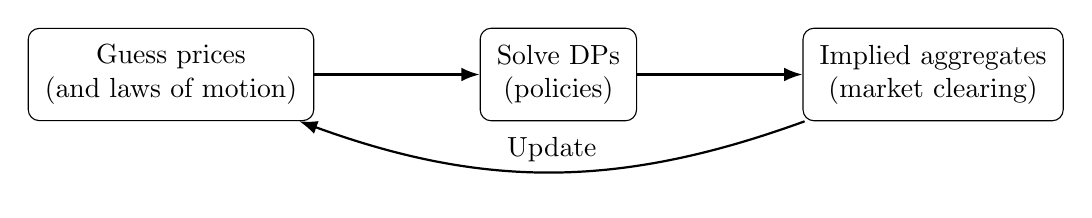
\begin{tikzpicture}[
  node/.style={rounded corners, draw, align=center, inner sep=6pt},
  arr/.style={-Latex, thick}
]
\node[node] (guess) {Guess prices\\(and laws of motion)};
\node[node, right=2.1cm of guess] (solve) {Solve DPs\\(policies)};
\node[node, right=2.1cm of solve] (imply) {Implied aggregates\\(market clearing)};
\draw[arr] (guess) -- (solve);
\draw[arr] (solve) -- (imply);
\draw[arr] (imply) to[bend left=20] node[above]{Update} (guess);
\end{tikzpicture}
\end{frame}

\begin{frame}{What ``learning DP'' really means in this class}

You will learn to:
\begin{itemize}
  \item Choose states that make the problem \textbf{Markov}
  \item Use Euler equations and envelopes to understand \textbf{margins}
  \item Compute policies using:
  \begin{itemize}
    \item value/policy iteration,
    \item discretization and simulation,
    \item (when appropriate) linearization
  \end{itemize}
\end{itemize}
\end{frame}

%========================================================================================
\section[1-sided]{One-sided labor search}
%========================================================================================

\begin{frame}{One-sided labor search (job search): why it matters}

Motivation:
\begin{itemize}
  \item Unemployment duration and wage dispersion can arise from \textbf{search frictions}
  \item Policy (benefits, taxes) works by shifting \textbf{accept/reject} incentives
\end{itemize}

\vspace{0.7em}
Key object:
\[
\text{Reservation wage } w^\star \quad \Rightarrow \quad
\text{accept if } w\ge w^\star.
\]
\end{frame}

\begin{frame}{Job search as a DP problem (structure, not details)}

State and choice:
\[
x_t \in \{\text{employment status},\ \text{offer }w_t\},\qquad
a_t \in \{\text{accept},\text{reject}\}.
\]

\vspace{0.5em}
Recursion creates:
\begin{itemize}
  \item an option value of waiting,
  \item a simple acceptance rule,
  \item predictions for hazards, durations, wage distributions.
\end{itemize}
\end{frame}

%========================================================================================
\section[2-sided]{Two-sided search and matching}
%========================================================================================

\begin{frame}{Two-sided search (DMP): why it matters}

Motivation:
\begin{itemize}
  \item Firms also search (vacancies), not just workers
  \item \textbf{Unemployment and vacancies} move in systematic ways
\end{itemize}

\vspace{0.8em}
Core objects:
\[
m(u,v)\ \text{(matching)},\qquad \theta=\frac{v}{u}\ \text{(tightness)}.
\]
\end{frame}

\begin{frame}{What DMP adds relative to job search}

Endogenous job creation:
\begin{itemize}
  \item Firms compare vacancy posting cost to expected hiring surplus
  \item Wages depend on surplus division (bargaining, wage posting, etc.)
\end{itemize}

\vspace{0.6em}
Quantitative payoffs:
\begin{itemize}
  \item Beveridge curve, job-finding rates, vacancy-filling rates
  \item Propagation of shocks through \(\theta\) (a key amplification margin)
\end{itemize}
\end{frame}

%========================================================================================
\section[Asset]{Asset pricing}
%========================================================================================

\begin{frame}{Asset pricing in macro: the price of risk}

Motivation:
\begin{itemize}
  \item Macro is not only quantities---prices contain information
  \item Risk premia reveal how agents value states of the world
\end{itemize}

\vspace{0.8em}
Central restriction:
\[
1=\E_t\!\left[M_{t+1} R_{t+1}\right],
\qquad M_{t+1}\ \text{(stochastic discount factor)}.
\]
\end{frame}

\begin{frame}{Why you should care (even if you ``don't do finance'')}

Asset pricing tools help you:
\begin{itemize}
  \item Diagnose what risks the economy is exposed to
  \item Measure how constraints/frictions change risk sharing
  \item Connect macro shocks to observed returns and spreads
\end{itemize}

\vspace{0.6em}
\small
Many modern papers combine: heterogeneous agents + incomplete markets + risk premia.
\end{frame}

%========================================================================================
\section[RBC]{Real business cycle}
%========================================================================================

\begin{frame}{RBC: the benchmark general equilibrium model}

Why RBC first:
\begin{itemize}
  \item A disciplined baseline: preferences, technology, market clearing
  \item Clear propagation: intertemporal substitution, capital accumulation
\end{itemize}

\vspace{0.8em}
Outcome:
\begin{itemize}
  \item A full set of equilibrium objects:
  \begin{itemize}
    \item policy functions, prices, aggregates,
    \item impulse responses and moments.
  \end{itemize}
\end{itemize}
\end{frame}

\begin{frame}{How RBC organizes your intuition}

RBC teaches you to separate:
\begin{itemize}
  \item \textbf{shocks} (what hits the economy),
  \item \textbf{propagation} (how the economy transmits shocks),
  \item \textbf{measurement} (what we call output, labor, productivity).
\end{itemize}

\vspace{0.6em}
Then we add frictions (search, heterogeneity, constraints) and see what changes.
\end{frame}

%========================================================================================
\section[Growth]{Endogenous growth}
%========================================================================================

\begin{frame}{Endogenous growth: where does the trend come from?}

Motivation:
\begin{itemize}
  \item Cycles fluctuate around a trend; growth determines long-run welfare
  \item Innovation/ideas create sustained growth, often with externalities
\end{itemize}

\vspace{0.7em}
Key deliverables:
\begin{itemize}
  \item Balanced growth paths and transitions
  \item Policy analysis: R\&D subsidies, education, market structure, IP
\end{itemize}
\end{frame}

%========================================================================================
\section[HA]{Heterogeneous agents}
%========================================================================================

\begin{frame}{Heterogeneous-agent macro: distribution as a state variable}

Motivation:
\begin{itemize}
  \item Inequality and imperfect insurance are first-order
  \item Many policies have strong \textbf{distributional} effects
\end{itemize}

\vspace{0.8em}
Core idea:
\begin{itemize}
  \item Individuals face idiosyncratic risk and incomplete markets
  \item Aggregate outcomes depend on the \textbf{wealth/income distribution}
\end{itemize}
\end{frame}

\begin{frame}{Why HA models changed modern macro}

They let you study:
\begin{itemize}
  \item MPCs and the power of redistribution/transfer policy
  \item Monetary/fiscal policy with heterogeneous balance sheets
  \item Labor-market risk interacting with saving and asset pricing
\end{itemize}

\vspace{0.6em}
\small
Computational skill: compute stationary distributions and transitions reliably.
\end{frame}

%========================================================================================
\section{Wrap-up}
%========================================================================================

\begin{frame}{Putting it together: the frontier is modular}

Modern research often combines modules:
\begin{itemize}
  \item Search frictions + HA \(\rightarrow\) unemployment risk, welfare, policy
  \item HA + asset pricing \(\rightarrow\) macro-finance with inequality
  \item RBC core + growth \(\rightarrow\) shocks, innovation, medium-run dynamics
\end{itemize}

\vspace{0.7em}
\small
The goal of this course is to make these combinations feel \textbf{natural}, not intimidating.
\end{frame}

\begin{frame}{How to succeed in this sequence}

\begin{itemize}
  \item Focus on \textbf{objects}: state, policy, price, distribution
  \item Always ask: \textbf{which margin moves?} \; (consumption/saving, vacancy posting, acceptance, pricing of risk)
  \item Treat computation as part of economics:
  \begin{itemize}
    \item if you can simulate it, you can measure it
    \item if you can measure it, you can test it
  \end{itemize}
\end{itemize}
\end{frame}

\end{document}
